\section{Complete Confirmatory Outcomes and Diagnostic Audit}
\label{app:complete-confirmation}

The frozen test contains 171 physical trajectories and 342 observed
records. Every method has an accounted output for every intended record;
the solver-rejection and inference-failure ledgers are empty. The
continuous, persistent-line and normal physical-parent counts are 18,
27 and 12. Three network conditions and two noise levels repeat these
parents. Normal controls are shared between evaluation lanes, not doubled
independent exposure. Tables below are generated directly from the sealed
summary, records, event matches and paired intervals.\AIDraftingCredit{}

\begin{table*}[t]\centering\small
\caption{Continuous outcomes by network and noise stratum. Each cell is timely family/source decisions / intended events; unmatched event-stream alarms. Replays share physical parents.}
\label{tab:review_continuous}
\begin{tabular}{llrrrr}\toprule
Network & Noise & Physical bank & Nominal bank & ExtraTrees & ET short\\\midrule
Matched & 1 & 108/108; 1 & 108/108; 1 & 56/108; 6 & 60/108; 5\\
Matched & 2 & 108/108; 0 & 108/108; 0 & 54/108; 4 & 58/108; 0\\
In-bank & 1 & 108/108; 2 & 108/108; 3 & 56/108; 5 & 60/108; 5\\
In-bank & 2 & 108/108; 1 & 108/108; 2 & 54/108; 4 & 57/108; 0\\
Out-of-bank & 1 & 106/108; 38 & 105/108; 47 & 56/108; 5 & 60/108; 6\\
Out-of-bank & 2 & 106/108; 30 & 106/108; 39 & 54/108; 5 & 57/108; 0\\
\bottomrule\end{tabular}
\end{table*}

\begin{table*}[t]\centering\small
\caption{Continuous monitoring: unavailable intended records, normal-record alarm incidence, normal alarm counts and available normal exposure, false restorations and open episodes. Counts combine six repeated strata descriptively; normal parents are not independent across strata. Missing outputs remain intended failures.}
\label{tab:c01_operational}
\begin{tabular}{lrrrrrr}\toprule
Method & Unavailable & Normal incidence & Normal alarms & Exposure (h) & False OFF & Open at end\\\midrule
Physical 5-model & 0 & 0/72 & 0 & 11.760 & 58 & 0\\
Physical nominal & 0 & 0/72 & 0 & 11.760 & 68 & 0\\
ExtraTrees & 0 & 0/72 & 0 & 11.760 & 29 & 0\\
ET short & 0 & 0/72 & 0 & 11.760 & 16 & 0\\
\bottomrule\end{tabular}\end{table*}

\begin{table*}[t]\centering\small
\caption{Conditional median diagnosis/restoration delays (s), kept within each paired stratum. These medians summarize matched emitted diagnoses/restoration messages with finite delay and must be read alongside omissions, unavailable records and censoring; -- denotes no finite estimate. Logical delays do not measure computational throughput.}
\label{tab:c01_delays}
\begin{tabular}{llrrrr}\toprule
R/X condition & Noise & Physical 5-model & Physical nominal & ExtraTrees & ET short\\\midrule
Matched & 1 & 0.27/0.18 & 0.27/0.18 & 0.23/0.18 & 0.19/0.18\\
Matched & 2 & 0.27/0.18 & 0.27/0.18 & 0.30/0.18 & 0.20/0.18\\
In-bank & 1 & 0.27/0.18 & 0.27/0.18 & 0.23/0.18 & 0.19/0.18\\
In-bank & 2 & 0.27/0.18 & 0.27/0.18 & 0.30/0.18 & 0.20/0.18\\
Out-of-bank & 1 & 0.33/0.18 & 0.33/0.18 & 0.23/0.18 & 0.19/0.18\\
Out-of-bank & 2 & 0.26/0.18 & 0.33/0.18 & 0.30/0.18 & 0.20/0.18\\
\bottomrule\end{tabular}\end{table*}

\begin{table*}[t]\centering\small
\caption{Persistent-line comparison on the common observations. Each cell gives correct first source / intended openings; pre-change stops / right-censored openings; mean restricted correct delay (s). Wrong first sources remain in the denominator. Restricted delay retains the horizon penalty for failures and censoring defined by the fixed evaluator.}
\label{tab:c01_first_stop}
\begin{tabular}{llrrr}\toprule
R/X condition & Noise & Physical 5-model & Physical nominal & Chen \emph{et al.}\\\midrule
Matched & 1 & 27/27; 0/0; 0.18 & 27/27; 0/0; 0.18 & 12/27; 11/0; 54.58\\
Matched & 2 & 27/27; 0/0; 0.18 & 27/27; 0/0; 0.18 & 12/27; 11/0; 54.58\\
In-bank & 1 & 27/27; 0/0; 0.18 & 27/27; 0/0; 0.18 & 13/27; 11/0; 51.04\\
In-bank & 2 & 27/27; 0/0; 0.18 & 27/27; 0/0; 0.18 & 13/27; 11/0; 51.05\\
Out-of-bank & 1 & 27/27; 0/0; 0.18 & 27/27; 0/0; 0.18 & 12/27; 11/0; 54.58\\
Out-of-bank & 2 & 27/27; 0/0; 0.18 & 27/27; 0/0; 0.18 & 12/27; 11/0; 54.59\\
\bottomrule\end{tabular}\end{table*}

\begin{table*}[t]\centering\small
\caption{Persistent-line coverage and stopping outcomes across six repeated strata, including both fixed ExtraTrees comparators. Normal controls are the same controls used in the continuous table, not additional exposure. Chen \emph{et al.} normal exposure ends at its first stop; the other methods monitor the full available record.}
\label{tab:c01_persistent_coverage}
\begin{tabular}{lrrrrrr}\toprule
Method & Unavailable & Correct first & Pre-change & Censored & Normal incidence & Exposure (h)\\\midrule
Physical 5-model & 0 & 162/162 & 0 & 0 & 0/72 & 11.760\\
Physical nominal & 0 & 162/162 & 0 & 0 & 0/72 & 11.760\\
ExtraTrees & 0 & 162/162 & 0 & 0 & 0/72 & 11.760\\
ET short & 0 & 162/162 & 0 & 0 & 0/72 & 11.760\\
Chen \emph{et al.} & 0 & 74/162 & 66 & 0 & 72/72 & 0.701\\
\bottomrule\end{tabular}\end{table*}


\subsection{Timely Coverage Versus Classification}
The additional confusion view in Fig.~\ref{fig:review-confusion} is a
posthoc descriptive audit. It uses the original evaluator's temporal
episode association and the first public diagnosis; it does not rematch
events using source labels. A diagnosis emitted after physical OFF is
counted as unavailable for this view. All diagnoses that are timely and
matched in these four procedures have the correct family and exact
source. The large load gap therefore reflects whether a diagnosis is
available before OFF, not a measured advantage in conditional label
accuracy among timely outputs. Unmatched alarms remain in the separate
alarm tables. Normal records are not mixed into this event-level matrix.

\begin{figure*}[t]\centering
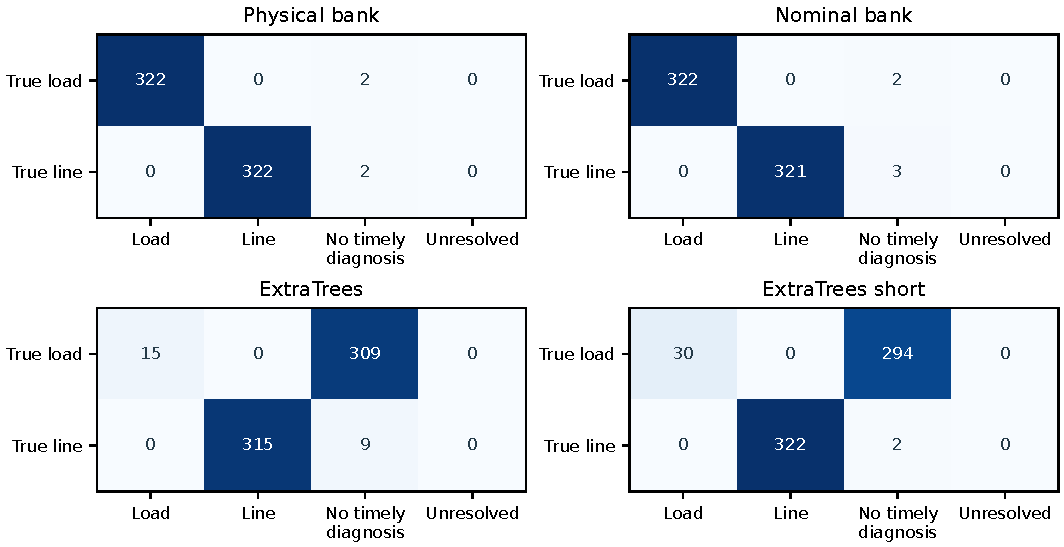
\includegraphics[width=.96\textwidth]{figures/generated/review_c01_confusion.pdf}
\caption{Posthoc confusion audit of the frozen continuous test, with 324
realizations per true family. No timely diagnosis includes omitted and
late diagnoses. Counts reuse the registered episode matches; all 432
prediction JSON files used were checked against the prediction seal.
These panels do not include unmatched alarms or constitute a new
predeclared endpoint.}
\label{fig:review-confusion}\end{figure*}

\begin{table*}[t]\centering\small
\caption{Timely decisions by source in the continuous test. These are correlated realizations of the registered physical schedules, not source-excluded generalization.}
\label{tab:review_sources}
\begin{tabular}{lrrrr}\toprule
Family / asset & Physical bank & Nominal bank & ExtraTrees & ET short\\\midrule
Line / LINE14-15 & 36/36 & 36/36 & 27/36 & 34/36\\
Line / LINE16-17 & 36/36 & 36/36 & 36/36 & 36/36\\
Line / LINE17-18 & 48/48 & 48/48 & 48/48 & 48/48\\
Line / LINE23-24 & 30/30 & 30/30 & 30/30 & 30/30\\
Line / LINE26-27 & 24/24 & 24/24 & 24/24 & 24/24\\
Line / LINE26-29 & 24/24 & 23/24 & 24/24 & 24/24\\
Line / LINE3-4 & 42/42 & 40/42 & 42/42 & 42/42\\
Line / LINE4-14 & 46/48 & 48/48 & 48/48 & 48/48\\
Line / LINE9-39 & 36/36 & 36/36 & 36/36 & 36/36\\
Load / BUS15 & 42/42 & 42/42 & 6/42 & 6/42\\
Load / BUS16 & 42/42 & 42/42 & 0/42 & 3/42\\
Load / BUS20 & 12/12 & 12/12 & 6/12 & 12/12\\
Load / BUS24 & 42/42 & 42/42 & 0/42 & 0/42\\
Load / BUS26 & 18/18 & 18/18 & 0/18 & 0/18\\
Load / BUS3 & 42/42 & 42/42 & 3/42 & 3/42\\
Load / BUS31 & 40/42 & 40/42 & 0/42 & 0/42\\
Load / BUS4 & 36/36 & 36/36 & 0/36 & 6/36\\
Load / BUS7 & 48/48 & 48/48 & 0/48 & 0/48\\
\bottomrule\end{tabular}
\end{table*}

\begin{table*}[t]\centering\small
\caption{Paired physical-bank minus learned-comparator differences. Timely attribution is in percentage points; extras are per full event-record hour, including startup. Brackets are the frozen 95-percent parent-bootstrap intervals.}
\label{tab:review_paired}
\begin{tabular}{ll ll rr}\toprule
Network & Noise & Method & Reference & Timely difference & Extra-rate difference\\\midrule
Matched & 1 & Physical bank & ExtraTrees short & 44.44 [40.48, 47.92] & -6.67 [-15.00, 0.00]\\
Matched & 1 & Physical bank & ExtraTrees & 48.15 [44.44, 51.67] & -8.33 [-18.33, 0.00]\\
Matched & 1 & Nominal bank & ExtraTrees short & 44.44 [40.74, 48.04] & -6.67 [-13.33, 0.00]\\
Matched & 1 & Nominal bank & ExtraTrees & 48.15 [44.44, 51.67] & -8.33 [-18.33, 0.00]\\
Matched & 2 & Physical bank & ExtraTrees short & 46.30 [42.75, 49.12] & 0.00 [0.00, 0.00]\\
Matched & 2 & Physical bank & ExtraTrees & 50.00 [46.30, 53.70] & -6.67 [-13.33, -1.67]\\
Matched & 2 & Nominal bank & ExtraTrees short & 46.30 [42.86, 49.12] & 0.00 [0.00, 0.00]\\
Matched & 2 & Nominal bank & ExtraTrees & 50.00 [46.38, 53.70] & -6.67 [-13.33, -1.67]\\
In-bank & 1 & Physical bank & ExtraTrees short & 44.44 [40.62, 47.92] & -5.00 [-13.33, 5.00]\\
In-bank & 1 & Physical bank & ExtraTrees & 48.15 [44.44, 51.67] & -5.00 [-13.33, 5.00]\\
In-bank & 1 & Nominal bank & ExtraTrees short & 44.44 [40.62, 47.92] & -3.33 [-11.67, 6.67]\\
In-bank & 1 & Nominal bank & ExtraTrees & 48.15 [44.44, 51.67] & -3.33 [-11.67, 5.00]\\
In-bank & 2 & Physical bank & ExtraTrees short & 47.22 [43.18, 50.98] & 1.67 [0.00, 5.00]\\
In-bank & 2 & Physical bank & ExtraTrees & 50.00 [46.49, 53.70] & -5.00 [-10.00, 0.00]\\
In-bank & 2 & Nominal bank & ExtraTrees short & 47.22 [43.33, 51.04] & 3.33 [0.00, 8.33]\\
In-bank & 2 & Nominal bank & ExtraTrees & 50.00 [46.30, 53.70] & -3.33 [-10.00, 3.33]\\
Out-of-bank & 1 & Physical bank & ExtraTrees short & 42.59 [38.60, 46.43] & 53.33 [36.67, 71.67]\\
Out-of-bank & 1 & Physical bank & ExtraTrees & 46.30 [42.11, 50.00] & 55.00 [36.67, 73.33]\\
Out-of-bank & 1 & Nominal bank & ExtraTrees short & 41.67 [36.11, 46.67] & 68.33 [46.67, 90.00]\\
Out-of-bank & 1 & Nominal bank & ExtraTrees & 45.37 [41.11, 50.00] & 70.00 [45.00, 95.00]\\
Out-of-bank & 2 & Physical bank & ExtraTrees short & 45.37 [41.11, 50.00] & 50.00 [35.00, 65.00]\\
Out-of-bank & 2 & Physical bank & ExtraTrees & 48.15 [43.59, 52.50] & 41.67 [25.00, 60.00]\\
Out-of-bank & 2 & Nominal bank & ExtraTrees short & 45.37 [41.11, 50.00] & 65.00 [41.67, 88.33]\\
Out-of-bank & 2 & Nominal bank & ExtraTrees & 48.15 [43.75, 52.56] & 56.67 [31.67, 80.00]\\
\bottomrule\end{tabular}
\end{table*}


\subsection{Maintaining a Sustained Event After the First Stop}
The first-stop score alone hides subsequent fragmentation. Although both
physical banks and both learned comparators correctly identify all 162
persistent openings first, the learned comparators later return to an
inactive label and issue additional alarms. Table~\ref{tab:review_persistence}
describes those already recorded outputs. It does not change the frozen
first-stop outcome or extend Chen's one-stop contract into a recurrent
monitor. Retained open episodes are appropriate when an intervention
continues beyond the record.
\begin{table*}[t]\centering\small
\caption{Descriptive persistence audit after first detection on sustained line openings. All four procedures first identify 162/162 lines. Extras are later unmatched alarms; unmatched OFF counts only restoration messages on unmatched episodes. Open-at-end messages are expected for sustained events and are not automatically errors. False-negative reports include detection delay and later inactive labels. Chen is a first-stop method and is excluded from this recurrent-monitoring diagnostic.}
\label{tab:review_persistence}
\begin{tabular}{lrrrrr}\toprule
Method & Openings & Extras & Unmatched OFF & Open at end & FN reports\\\midrule
Physical bank & 162 & 0 & 0 & 162 & 810\\
Nominal bank & 162 & 0 & 0 & 162 & 810\\
ExtraTrees & 162 & 164 & 164 & 16 & 335374\\
ExtraTrees short & 162 & 179 & 178 & 61 & 182600\\
\bottomrule\end{tabular}
\end{table*}


\subsection{Measurement Integrity Is a Separate Executed Component}
\begin{table*}[t]\centering\small
\caption{Retrospective measurement-integrity components over 180 windows. Hits require family and PMU identity. Missingness is observed availability; corrupted-data identification is inherited from the window classifier. These are not counts of attributed cyberattacks.}
\label{tab:review_integrity}
\begin{tabular}{lrrr}\toprule
Component & Positive-window hits & FP & FN\\\midrule
Missing & 14/14 & 0 & 0\\
Corrupt & 1/2 & 2 & 1\\
\bottomrule\end{tabular}
\end{table*}

The availability interface correctly identifies all four missing-data
intervals at the first received report that reveals the loss. This is a
received-report clock, not zero transport or computation latency.
Bad-data labels come from the inherited window classifier. Neither
missingness nor corruption proves malicious intent. The composition
preserves physical-source and affected-PMU identities but does not run a
joint physical/cyber Bayesian filter; the physical bank is unavailable on
the retrospective RAW0001 replay under its startup noise-scale contract.

\FloatBarrier
